\section{Related Work}  
\subsection{Coreset Selection}  
Coreset selection identifies a representative subset from the original (noisy) dataset with the objective of increasing training efficiency or enhancing model effectiveness. Recent methods are categorized into optimization-based and heuristic-based. Optimization-based approaches employ bilevel optimization~\cite{borsos2020coresets,zhou2022probabilistic,hao2024bilevel} or gradient matching objectives~\cite{killamsetty2021grad,mirzasoleiman2020coresets,killamsetty2021glister,killamsetty2021retrieve}, providing theoretical guarantees, but incurring high costs. Heuristic-based methods assess sample importance via forgetting events~\cite{toneva2018empirical}, gradient~\cite{pruthi2020estimating,xia2024less,thakkar2023self}, and inter-sample distances~\cite{xia2022moderate}. Recent progress includes DNN-based selectors~\cite{ilyas2022datamodels,engstrom2024dsdm} and efficient frameworks~\cite{everaert2023gio,paul2021deep,xiao2024feature,park2024robust} that balance quality and efficiency.

\begin{figure*}[!htbp]
  \centering
  \begin{subfigure}{0.32\linewidth}
    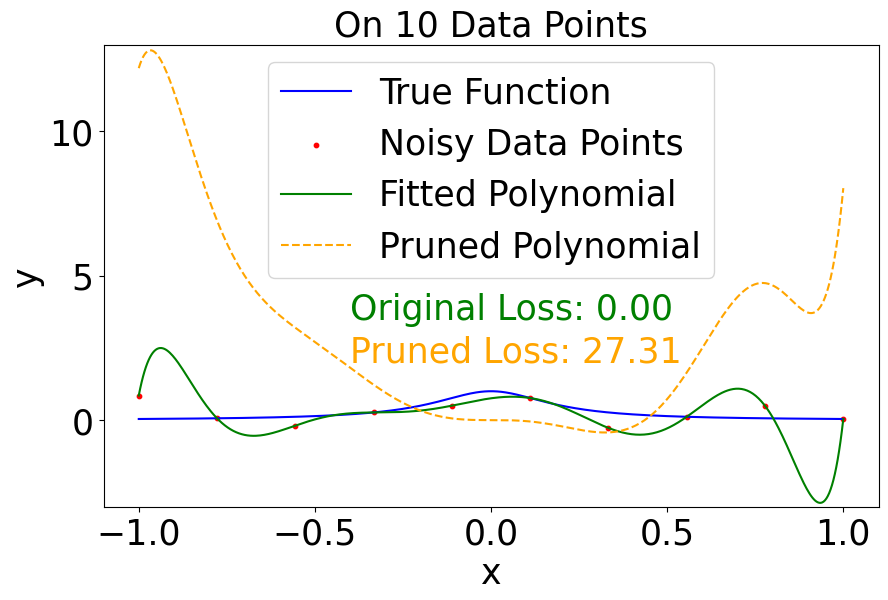
\includegraphics[width=1.0\linewidth]{figs/poly_fit_noise_n10.png}
    \caption{On noisy samples}
    \label{fig:fit_10}
  \end{subfigure}
  \hfill
  \begin{subfigure}{0.32\linewidth}
    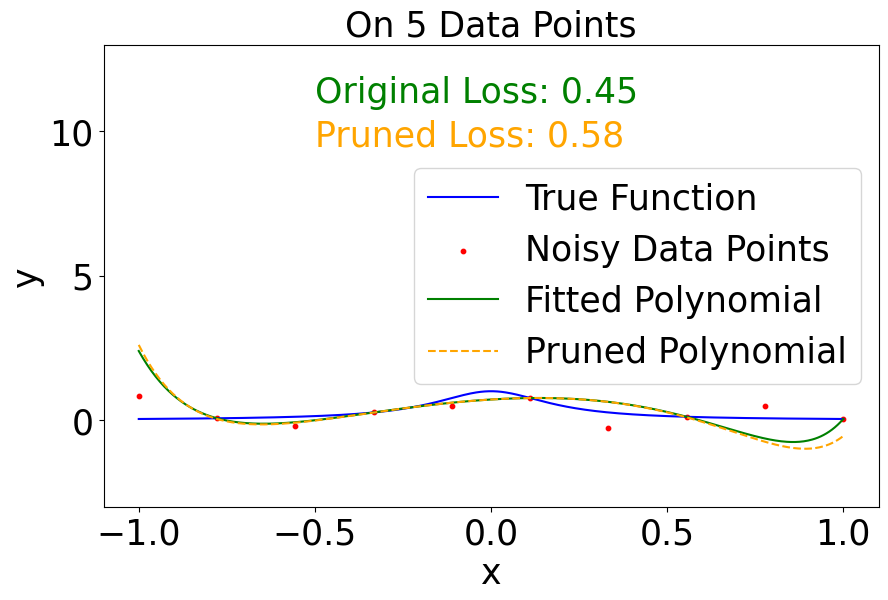
\includegraphics[width=1.0\linewidth]{figs/poly_fit_noise_n5.png}
    \caption{On clean samples}
    \label{fig:fit_5}
  \end{subfigure}
  \hfill
  \begin{subfigure}{0.32\linewidth}
    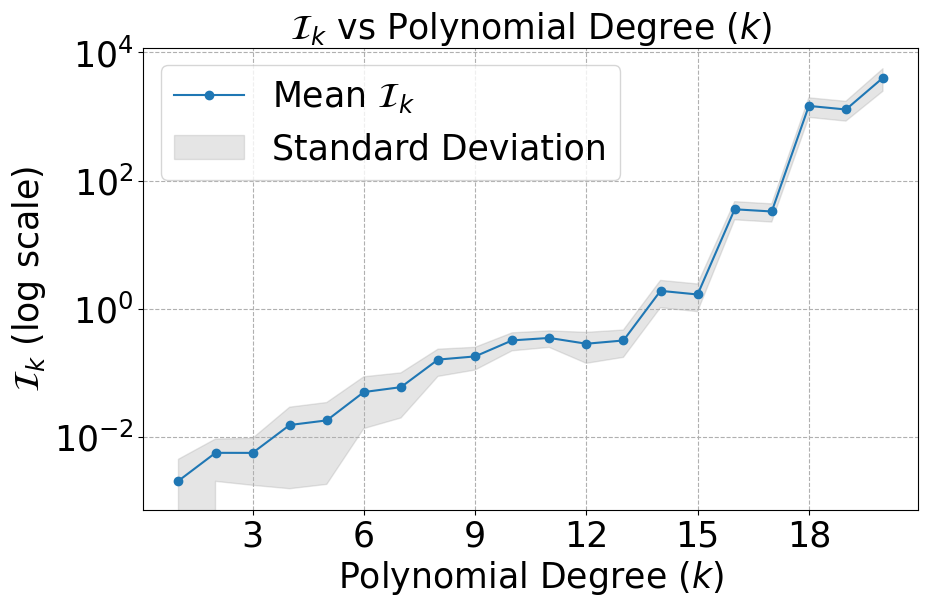
\includegraphics[width=1.0\linewidth]{figs/epsilon_vs_degree.png}
    \caption{\( \mathcal{I}(\mathcal{D}, \hat{\mathcal{D}}) \) values}
    \label{fig:epsilon}
  \end{subfigure}
  \caption{\textbf{The impact of redundant weights and samples on pruning and coreset selection.} 
  The collapsed pruned model ({\color{orange} yellow curve}) in (a) compared to (b) implies that noisy/redundant data increases the difficulty of pruning.
  (c) shows selection difficulty \( \mathcal{I}(\mathcal{D}, \hat{\mathcal{D}}) \) rises with polynomial degree, indicating harder coreset selection.}
  \label{fig:poly}
\end{figure*}

\subsection{Weight Pruning}  
Weight pruning is a key technique for model compression and acceleration, classified into structured and unstructured methods. Structured pruning methods~\cite{filterspruning,he2018soft,jiang2022channel,elkerdawy2022fire,guan2022dais,nonnenmacher2021sosp,alvarez2016learning,murray2015auto} remove entire filters or channels, enabling hardware acceleration but often reducing accuracy. In contrast, unstructured pruning~\cite{tanaka2020pruning,lee2018snip,han2015deep,frankle2018lottery} eliminates individual weights based on metrics like magnitude or gradient sensitivity~\cite{evci2020rigging,han2015learning,wen2016learning,blakeney2020pruning,renda2020comparing,hassibi1992second,lecun1989optimal}. Recent theoretical work link pruning to optimization theory~\cite{grosse2016kronecker,zhou2021effective,srinivas2017training,louizos2017learning,qian2021probabilistic}, bolstering its foundations.

\subsection{Pruning and Coreset Selection in Classical ML}
In classical machine learning, feature and sample screening mirror weight pruning and coreset selection. Optimization-based theoretical frameworks exist for joint feature and sample screening in this domain~\cite{shibagaki2016simultaneous,zhang2017scaling}. Empirically, feature screening enhances sample importance estimation, and vice versa. While these theories don't translate directly to deep learning, this synergy motivates integrating weight pruning and coreset selection.